\documentclass{standalone}
\usepackage{tikz, xcolor}
\usetikzlibrary{shapes,arrows}

\begin{document}

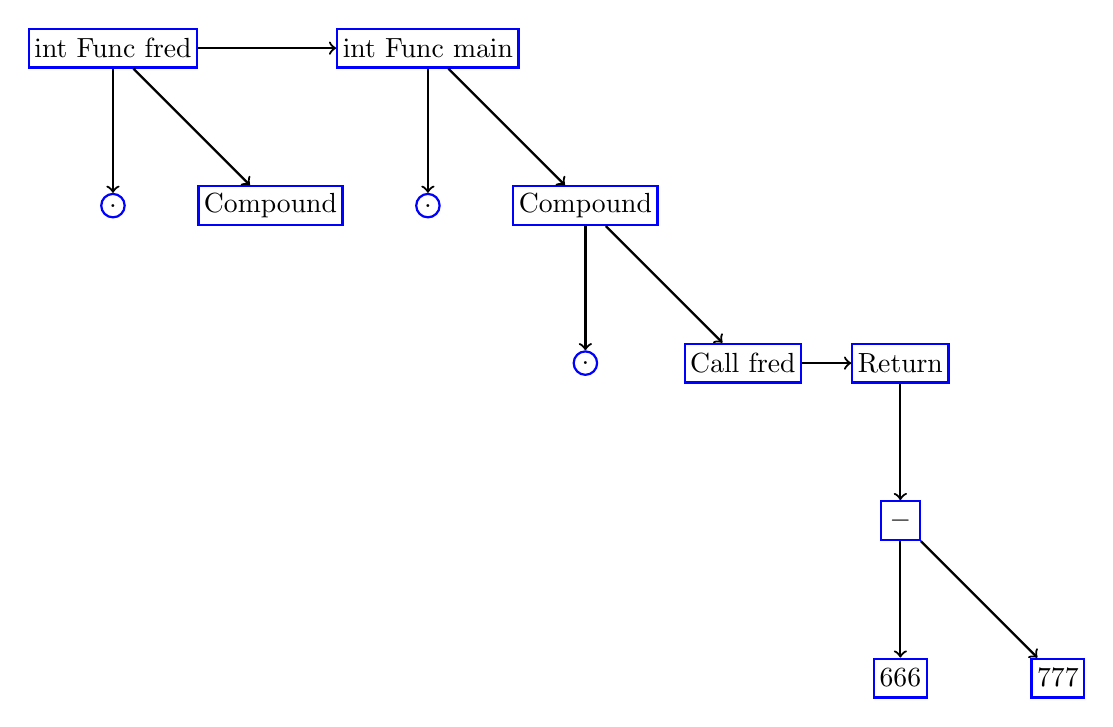
\begin{tikzpicture}[thick, scale=2.0]
\tikzstyle{vertexr}=[rectangle, draw=blue, thick, minimum size=14pt, inner sep=2pt]
\tikzstyle{vertexc}=[circle, draw=blue, thick, inner sep=2pt]
\tikzstyle{drawstyle}=[thick, ->]

\node[vertexr] (G0x0) at (0,0) {int Func fred};
\node[vertexc] (G0x1) at (0,-1) {.};
\draw[drawstyle] (G0x0) -- (G0x1);
\node[vertexr] (G1x1) at (1,-1) {Compound};
\draw[drawstyle] (G0x0) -- (G1x1);
\node[vertexr] (G2x0) at (2,0) {int Func main};
\node[vertexc] (G2x1) at (2,-1) {.};
\draw[drawstyle] (G2x0) -- (G2x1);
\node[vertexr] (G3x1) at (3,-1) {Compound};
\node[vertexc] (G3x2) at (3,-2) {.};
\draw[drawstyle] (G3x1) -- (G3x2);
\node[vertexr] (G4x2) at (4,-2) {Call fred};
\node[vertexr] (G5x2) at (5,-2) {Return};
\node[vertexr] (G5x3) at (5,-3) {$-$};
\node[vertexr] (G5x4) at (5,-4) {666};
\draw[drawstyle] (G5x3) -- (G5x4);
\node[vertexr] (G6x4) at (6,-4) {777};
\draw[drawstyle] (G5x3) -- (G6x4);
\draw[drawstyle] (G5x2) -- (G5x3);
\draw[drawstyle] (G4x2) -- (G5x2);
\draw[drawstyle] (G3x1) -- (G4x2);
\draw[drawstyle] (G2x0) -- (G3x1);
\draw[drawstyle] (G0x0) -- (G2x0);
\end{tikzpicture}
\end{document}
WARNING(1): Expecting to return type int but function 'fred' has no return statement.
Number of warnings: 1
Number of errors: 0
